\documentclass[11pt,a4paper]{article}

% -----------------------------------------------------------------------------
% CS6868 Research Mini-Project Report Template
% -----------------------------------------------------------------------------
% Target length: 5-10 pages (including figures, excluding references).
% Compile with: latexmk -pdf main.tex
% -----------------------------------------------------------------------------

\usepackage[utf8]{inputenc}
\usepackage[T1]{fontenc}
\usepackage[margin=1in]{geometry}
\usepackage{microtype}
\usepackage{lmodern}
\usepackage{amsmath,amssymb}
\usepackage{graphicx}
\graphicspath{{figures/}}
\usepackage{booktabs}
\usepackage{array}
\usepackage{enumitem}
\usepackage{xcolor}
\usepackage{listings}
\usepackage{hyperref}
\usepackage[capitalise,noabbrev]{cleveref}

\hypersetup{
  colorlinks=true,
  linkcolor=black,
  citecolor=blue!60!black,
  urlcolor=blue!60!black,
}

% Hyperlink short commit hashes to GitHub.
\newcommand{\commit}[1]{%
  \href{https://github.com/durwasa-chakraborty/CS6868_Concurrent_Programming_Project/commit/#1}%
       {\texttt{#1}}}

%Allow paragraph reflow to absorb long \texttt{...} identifiers without
% overfull hboxes. \sloppy prefers wider inter-word glue over margin
% violations; \emergencystretch raises the threshold; xurl lets URLs and
% path-like identifiers break at any character.
\usepackage{xurl}
\setlength{\emergencystretch}{5em}
\sloppy

%-Listings style (for code snippets) ---------------------------------------
\definecolor{codegray}{gray}{0.95}
\lstset{
  basicstyle=\ttfamily\small,
  backgroundcolor=\color{codegray},
  frame=single,
  framesep=4pt,
  breaklines=true,
  columns=fullflexible,
  keepspaces=true,
  showstringspaces=false,
}

%-Title block --------------------------------------------------------------
\title{%
  \textbf{CS6868 Research Mini-Project} \\[0.3em]
  \Large Segment Queue Synchronizer%
}
\author{%
  Mitesh Sharma \\ \texttt{cs25s011@smail.iitm.ac.in}
  \and
  Navaneeth M. Nambiar \\ \texttt{ns26z081@smail.iitm.ac.in}
  \and
  Durwasa Chakraborty \\ \texttt{cs24d011@smail.iitm.ac.in}
}
\date{\today}

\begin{document}
\maketitle


\begin{abstract}
Writing concurrent code with ensured correctness and performance is a
notoriously tough task. CancellableQueueSynchronizer
(CQS)~\cite{koval2023cqs} is a new experimental framework enabling simple
and efficient implementations of such synchronization primitives for
Kotlin coroutines. It emphasises rich semantics for lightweight threads
that are cheap to suspend and resume while supporting fair FIFO ordering
and abortable operations, all backed by modular formal proofs of their
properties. We port the Cancellable Queue Synchronizer
(CQS)~\cite{koval2023cqs} from Kotlin to
OCaml~5~\cite{kcsrk2020}. Each primitive is tested against a hand-written
2-domain linearizability harness, with \texttt{qcheck-lin}~\cite{qcheck},
\texttt{qcheck-stm}, and with manual cross-domain scenarios under
ThreadSanitizer; all pass. We benchmark against
\texttt{java.util.concurrent.AbstractQueueSynchronizer}~\cite{lea2005aqs}
on 1--8 threads. Our implementations of blocking pools and count-down
latch beat Java, but our mutex and semaphore are slower under contention
because Eio fibre park/wake costs more than a JVM thread context switch.
While the results were mixed, we highlight a faster feedback loop porting
code and the need for good abstractions and advanced testing.
\end{abstract}

% =============================================================================
\section{Goals}
\label{sec:goals}
% =============================================================================

Our main objective is to port the Cancellable Queue Synchronizer
(CQS)~\cite{koval2023cqs} framework, originally written for Kotlin
coroutines, to OCaml~5~\cite{kcsrk2020}. The highlights of CQS are:

\begin{itemize}[leftmargin=1.5em,nosep]
  \item Simple semantics for suspending and resuming coroutines.
  \item Expressive power capable of implementing mutexes, semaphores,
        barriers, and count-down latches.
  \item Formal proofs of its properties in Rocq.
\end{itemize}

Being able to do this on a common abstraction keeps things relatively
simple and allows for modularity and code reuse across primitives that
would otherwise each ship a bespoke wait-queue. Because CQS is already
implemented in Kotlin, it is also a good candidate for understanding the
use case of agentic AI in porting between languages while leveraging the
existing tests as a correctness oracle.

In particular, CQS incorporates multiple aspects such as:

\begin{itemize}[leftmargin=1.5em,nosep]
  \item Matching suspend and resume operations similarly to how push
        and pop operations are matched in an elimination stack.
  \item A \emph{helping} mechanism for handling cancelled coroutines, so
        that a single \texttt{resume} can absorb a run of cancellations
        rather than retrying once per cancelled cell.
\end{itemize}

\paragraph{Research question}
Would a similar framework benefit an OCaml-5-native concurrency model
built on Eio fibres~\cite{eio}? How do our primitive implementations
compare against Java's \texttt{java.util.concurrent}~\cite{lea2005aqs}
and Kotlin's \texttt{kotlinx.coroutines.sync}, and how can we confirm
this quantitatively?

% =============================================================================
\section{Background}
\label{sec:background}
% =============================================================================


\subsection{Motivation: Fairness, Abortability, and the Coroutine Setting}
\label{sec:bg-motivation}

Synchronization primitives like mutexes, semaphores, barriers, etc.\ are
among the most fundamental abstractions in concurrent programming. Modern
programming languages therefore require strong semantics and formal
guarantees from them.

Two properties are particularly desirable.
(a) \textbf{Fairness}: waiting requests should be served in the order
of their arrival (FIFO), preventing starvation.
(b) \textbf{Abortability}: a waiting request must be cancellable at
        any time, due to a timeout or an explicit user action.

These requirements have become especially pressing with the rise of
\emph{coroutines}, which are lightweight scheduling units that can be
spawned in large numbers within a single process, are cheaper to suspend
and resume than native threads, and are more frequently cancelled. When a
coroutine suspends, its underlying thread immediately picks up another
coroutine rather than blocking. Hence, the cost of fair scheduling is
lower than in a thread-based model, while the cost of inefficient
cancellation is higher.

The only practical abstraction that provides similar semantics prior to
this work is Java's \texttt{AbstractQueuedSynchronizer}
(AQS)~\cite{lea2005aqs}, which forms the core of the
\texttt{java.util.concurrent} package. AQS maintains a CLH-style
doubly-linked queue of waiting threads and uses CAS on an integer state
field. Cancelling a thread in AQS requires traversing the queue linearly
and unlinking a cancelled node. While this is fine for a small number of
threads, it does not scale well for large numbers of lightweight
coroutines that may be cancelled more frequently.

\subsection{The CQS Framework}
\label{sec:bg-cqs}

Koval et~al.~\cite{koval2023cqs} introduce the \textbf{Cancellable Queue
Synchronizer} (CQS) to close this gap. CQS provides two operations:
\begin{itemize}[leftmargin=1.5em,nosep]
  \item \texttt{suspend()}: adds the current thread (or coroutine) as a
        waiter and suspends.
  \item \texttt{resume(result)}: retrieves and resumes the next waiter,
        passing it the specified value.
\end{itemize}

Here, \texttt{resume()} may be called \emph{before} \texttt{suspend()}.
If a \texttt{resume()} arrives at a cell before the matching
\texttt{suspend()}, the value is deposited in the cell and the later
\texttt{suspend()} claims it atomically and returns immediately without
actually suspending-an \emph{elimination}. Primitive implementations
exploit this property for both simplicity and performance.

\subsection{Asynchronous Resume and Suspend}
\label{sec:bg-async}

In a sequential setting, a resume operation coming before a suspend
cannot be linearized appropriately. However, in a concurrent setting we
need to allow such an execution for high throughput. This implies that a
resume operation entering a CQS may be valid as long as a concurrent
suspend is available to satisfy it. This is the core idea behind the
SYNC/ASYNC modes of CQS operations.

\subsection{Cancellation Support}
\label{sec:bg-cancel}

Supporting cancellation without races is the central technical challenge
of CQS. The framework defines two modes for this:

\begin{enumerate}[leftmargin=1.5em]
  \item \textbf{Simple cancellation.} When a waiter is cancelled, its
        cell is marked \texttt{CANCELLED}. A \texttt{resume()} that
        encounters a \texttt{CANCELLED} cell simply returns
        \texttt{false}, signalling to the calling primitive that it must
        retry. This mode is straightforward but has a linear-time worst
        case when many consecutive waiters are cancelled before the
        corresponding \texttt{resume()} arrives: each \texttt{resume()}
        must traverse all cancelled cells individually.

  \item \textbf{Smart cancellation.} Smart cancellation allows
        \texttt{resume()} to skip cancelled cells and retry atomically,
        reducing the cost of a sequence of cancellations per
        \texttt{resume()}. Intuitively, the difference is that in the
        simple cancellation mode \texttt{resume(\ldots)} fails if the
        thread in the corresponding cell has been cancelled, whereas
        smart cancellation enables efficient skipping of a sequence of
        aborted requests.
\end{enumerate}

\subsection{Synchronization Primitives Built on CQS}
\label{sec:bg-primitives}

The paper demonstrates the expressiveness of the framework by building
five primitives on top of it.

\paragraph{Mutex and Semaphore.}
Implemented with a signed integer counter. A non-positive counter
encodes the number of waiting \texttt{lock()} callers; a positive value
encodes the number of available permits.
\texttt{lock()}/\texttt{acquire()} decrements the counter via
Fetch-And-Add (FAA); if the pre-decrement value was positive, the
operation succeeds immediately, otherwise it calls \texttt{suspend()}.
\texttt{unlock()}/\texttt{release()} increments the counter via FAA; if
the pre-increment value was negative there is a waiter, and
\texttt{resume()} is called. When in Smart cancellation mode,
\texttt{onCancellation()} increments the counter and returns
\texttt{true} if the counter was still negative (waiter successfully
removed), or \texttt{false} if the counter reached zero or above (a
concurrent \texttt{resume()} is incoming and must be refused).

\paragraph{Barrier.}
Maintains a \texttt{remaining} counter initialized to the number of
coroutines. Each \texttt{arrive()} decrements \texttt{remaining} via
FAA. All coroutines except the last caller will get suspended; the last
caller issues $\textit{coroutines} - 1$ \texttt{resume()} calls to wake
up all the others. Cancellation is not supported: cancelling a coroutine
that has already physically reached the barrier point should not block
the remaining coroutines, so cancelled waiters are silently ignored via
smart cancellation.

\paragraph{Count-Down Latch.}
Maintains two counters: \texttt{count} (remaining \texttt{countDown()}
calls) and \texttt{waiters} (number of suspended \texttt{await()}
callers). When the latch fires, a special \texttt{DONE\_BIT} is set
atomically by the thread that drives \texttt{count} to zero, signalling
that the latch has fired. Afterwards, \texttt{await()} checks this bit
and returns immediately if the latch has already fired.

\paragraph{Blocking Pools (queue and stack variants).}
Transfer actual elements through CQS rather than unit tokens. Combine an
FAA-based availability counter with a flat array (FIFO) or a Treiber
stack (LIFO). \texttt{put()} increments the counter; if negative it
calls \texttt{resume(element)} directly. \texttt{retrieve()} decrements
the counter; if positive it pops an element, otherwise it calls
\texttt{suspend()}. Neither variant is linearizable-concurrent races
can produce non-FIFO or non-LIFO delivery-but this matches practical
pool semantics where elements are interchangeable resources.


% =============================================================================
\section{Tasks Undertaken}
\label{sec:tasks}
% =============================================================================

\subsection{Implementation}
\label{sec:tasks-impl}

Our implementation is split into two layers:
(a) a domain-safe suspendable fibre layer
(\texttt{lib/light\_thread.ml}); and
(b) the core CQS engine (\texttt{lib/sqs\_effects.ml}).
On top of these, we built six synchronization primitives in
\texttt{implementations/}: \texttt{Mutex}, \texttt{Semaphore},
\texttt{Barrier}, \texttt{CountDownLatch}, \texttt{BlockingQueuePool},
and \texttt{BlockingStackPool}.

\subsubsection{Domain-Safe Fibre: \texttt{Light\_thread}}
\label{sec:impl-light-thread}

The decision to implement light-weight threads as a stand-in for Kotlin
coroutines was directly inspired by the lectures in class, where we
implemented a similar go-routine mechanism on top of OCaml~5
effect handlers~\cite{kcsrk2020}. The first design decision was how to
represent a suspended fibre. An early prototype (commit
\commit{ecb5855}) used raw OCaml~5 effect handlers and stored suspended
fibres as \texttt{Effect.Deep.continuation} values. However, deeper
inspection revealed a critical issue with this approach.

\paragraph{OCaml~5 continuations are domain-local.}
The OCaml~5 runtime stores a pointer into the \emph{originating}
domain's stack, so calling \texttt{Effect.Deep.continue~k~v} from a
different domain is undefined behaviour. This made it impossible to
have one domain call \texttt{acquire} while another calls
\texttt{release}, which would have made all concurrent implementations
incorrect. The constraint becomes especially problematic when
implementing the \texttt{cancel} API call for a fibre, since
cancellation is fundamentally a cross-domain interaction.

To deal with this limitation, the final design (commit \commit{17adae2})
replaces raw effect handlers with Eio's fibre scheduler~\cite{eio}.
The Eio runtime guarantees that the wake-up function it hands back to
us is safe to call from any domain or systhread. The key type is:

\noindent\begin{minipage}{\linewidth}
\begin{lstlisting}[language=Caml]
(* lib/light_thread.ml, line 57 *)
type 'a t = ('a, exn) result -> unit
\end{lstlisting}
\end{minipage}

A suspended fibre is therefore a heap-allocated, domain-safe
\emph{enqueue function}. Calling it with \texttt{Ok~v} schedules the
fibre to resume with value \texttt{v}, mapping back to
\texttt{resume(v)}. Calling it with \texttt{Error~e} schedules it to
resume by raising \texttt{e}, mapping back to \texttt{cancel(exn)}.
The three primitives built on top are:

\noindent\begin{minipage}{\linewidth}
\begin{lstlisting}[language=Caml]
let suspend register =
  Eio.Private.Suspend.enter "sqs_suspend"
    (fun _ctx enqueue -> register enqueue)

let resume      (t : 'a t) (v : 'a)  : unit = t (Ok v)
let discontinue (t : 'a t) (e : exn) : unit = t (Error e)
\end{lstlisting}
\end{minipage}

\subsubsection{Core SQS Data Structures}
\label{sec:impl-sqs-data}

\paragraph{Segment.}
Waiters are stored in an unbounded doubly-linked list of
\emph{segments}, each holding exactly $16$ cells:

\noindent\begin{minipage}{\linewidth}
\begin{lstlisting}[language=Caml]
'a segment = {
  id              : int;
  cells           : 'a cell_state Atomic.t array;  (* 16 cells *)
  next            : 'a segment option Atomic.t;
  prev            : 'a segment option Atomic.t;
  cancelled_count : int Atomic.t;
  pointers        : int Atomic.t;
}
\end{lstlisting}
\end{minipage}

The fields are:
(a) \texttt{cells}: array storing the cells in the segment;
(b) \texttt{next}: the next segment in the infinite queue;
(c) \texttt{prev}: the previous segment in the infinite queue;
(d) \texttt{cancelled\_count}: tracks how many cells in the segment have
been cleaned up;
(e) \texttt{pointers}: a lightweight reference count for the two SQS
head/tail pointers (\texttt{resume\_segment}, \texttt{suspend\_segment})
that may still be pointing at the segment.

The doubly-linked layout is purely an implementation detail enabling
fast unlinking of segments whose cells have all been cancelled or
refused.

\paragraph{Cell State Machine.}
A cell slot in a segment is initially \texttt{Empty} and transitions through one of ten states: \texttt{Empty}, \texttt{Waiter} (a live fibre is parked), \texttt{Cancelling} (transient state during cancellation), \texttt{Cancelled}, \texttt{Refuse} (cell refuses the next \texttt{resume}), \texttt{Resumed} (continuation handed off), \texttt{Taken} (value grabbed by a concurrent suspend), \texttt{Broken} (a SYNC resume timed out), \texttt{Value} (resume deposited a value before suspend), and \texttt{WrappedValue} (as \texttt{Value}, but distinguishable from \texttt{Waiter}). From \texttt{Empty}, the cell transitions to \texttt{Value} if a \texttt{resume} arrives first, or to \texttt{Waiter} if a \texttt{suspend} arrives first. In the former case, the deposited value is later claimed by the paired \texttt{suspend} via the elimination path; CQS~\cite{koval2023cqs} supports both \texttt{Async} mode (resume returns immediately after depositing) and \texttt{Sync} mode (resume busy-waits for a bounded window, marking the cell \texttt{Broken} on timeout), and all six primitives use \texttt{Async} since operations like \texttt{release} or \texttt{count\_down} need not block on a handshake. In the latter case, a parked \texttt{Waiter} either reaches \texttt{Resumed} when a matching \texttt{resume} arrives (resumption path), or transitions to \texttt{Cancelled} or \texttt{Refuse} when a \texttt{cancel} request fires on the parked fibre, depending on the cancellation mode (see \cref{sec:impl-cancel}); the terminal states reachable along these paths are described in \cref{sec:impl-sqs-data,sec:impl-cancel} and illustrated in \cref{fig:cell-state}.
\texttt{Waiter}.

\begin{figure}[htbp]
  \centering
  \includegraphics[width=0.9\linewidth]{state_diagram.png}
  \caption{Cell state machine. From the initial \texttt{Empty} state a
  cell either transitions to \texttt{Value} (resume arrives first) or
  \texttt{Waiter} (suspend arrives first), and from there to one of
  the terminal states (\texttt{Resumed}, \texttt{Taken},
  \texttt{Cancelled}, \texttt{Refuse}, or \texttt{Broken}) via the
  paths described in \cref{sec:impl-sqs-data,sec:impl-cancel}.}
  \label{fig:cell-state}
\end{figure}



\paragraph{SQS Record.}
\label{sec:impl-sqs-record}
The top-level SQS handle is a record of atomic cursors and primitive
hooks:

\noindent\begin{minipage}{\linewidth}
\begin{lstlisting}[language=Caml,basicstyle=\ttfamily\footnotesize]
(* sqs_effects.ml, lines 109--119 *)
and 'a t = {
  resume_segment           : 'a segment Atomic.t;
  resume_idx               : int Atomic.t;
  suspend_segment          : 'a segment Atomic.t;
  suspend_idx              : int Atomic.t;
  resume_mode              : resume_mode;       (* Sync | Async *)
  cancellation_mode        : cancellation_mode; (* Simple | Smart *)
  on_cancellation          : unit -> bool;
  try_return_refused_value : 'a -> bool;
  return_value             : 'a -> unit;
}
\end{lstlisting}
\end{minipage}

Two pairs of \texttt{(segment, idx)} fields maintain independent
cursors for the resumer (front) and the suspender (back). Both indices
advance monotonically with Fetch-And-Add, which ends up being the only
atomic read-modify-write primitive needed to claim a cell.

\subsubsection{Cancellation Procedure and Modes}
\label{sec:impl-cancel}

Cancellation uses a two-phase protocol to prevent races with concurrent
\texttt{resume} calls. Phase~1 (\texttt{try\_mark\_cancelling},
\texttt{lib/sqs\_effects.ml:422--434}) CAS-es the cell from
\texttt{Waiter} to \texttt{Cancelling}; if it has already been
\texttt{Resumed}, cancellation loses the race and the fibre receives
the value normally. Phase~2 (\texttt{handle\_cancellation},
\texttt{lib/sqs\_effects.ml:460--489}) installs the final state under
one of CQS's two cancellation modes~\cite{koval2023cqs}: \textbf{Simple}
marks the cell \texttt{Cancelled} and lets future \texttt{resume}s skip
it, with segments unlinked once all slots are dead; \textbf{Smart}
invokes an \texttt{on\_cancellation()} handler --- on \texttt{true} the
cell is \texttt{Cancelled} but any value stranded mid-\texttt{Cancelling}
is forwarded with a fresh \texttt{resume} so no permits leak, and on
\texttt{false} it is \texttt{Refuse}d, with the next arriving value
rerouted back into the data structure via
\texttt{try\_return\_refused\_value}. The transient \texttt{Cancelling}
state serialises against \texttt{Async} resumers, which CAS against the
live \texttt{Cancelling~k} pointer and may deposit a value the handler
later reads back via \texttt{Atomic.exchange} in \texttt{mark\_impl}.

\subsubsection{Key Atomic Operations}
\label{sec:impl-atomics}

The implementation uses three atomic operations from OCaml~5's
\texttt{Atomic} module:

\begin{center}\small
\begin{tabular}{@{}p{0.42\linewidth}p{0.50\linewidth}@{}}
\toprule
\textbf{Operation} & \textbf{Used for} \\
\midrule
\texttt{Atomic.fetch\_and\_add idx 1}
  & Claiming the next cell index (suspend / resume cursors) \\
\texttt{Atomic.compare\_and\_set} \newline
\texttt{\ \ cell expected desired}
  & All cell-state transitions; segment linking; done-bit install \\
\texttt{Atomic.exchange cell new\_state}
  & Cancellation finalisation (\texttt{mark\_impl}) \\
\bottomrule
\end{tabular}
\end{center}

\texttt{fetch\_and\_add} on the cursor is the only operation that must
succeed unconditionally, ensuring every caller receives a unique index.
All subsequent cell operations are CAS-based and retry on conflict.
\texttt{Atomic.exchange} is used during cancellation finalisation
because the old state of the cell needs to be atomically replaced
\emph{while} its value is being inspected; a CAS-loop here would create
a window in which a concurrent \texttt{resume} could insert a value
between the read and the swap.

Every shared variable in the CQS implementation is either an
\texttt{Atomic.t} or immutable. Correctness relies entirely on the
CAS/FAA-based state machines described above, matching the lock-free
design of the original CQS algorithm~\cite{koval2023cqs}.

\paragraph{The Physical-Equality Invariant.}
A critical invariant pervades every CAS in our implementation:
\emph{always CAS against a heap pointer read in the same critical
region, never against a freshly reconstructed value of the same shape.}
OCaml's \texttt{Atomic.compare\_and\_set} requires \emph{physical}
equality (\texttt{==}), not structural equality (\texttt{=}), for a
successful CAS. A freshly allocated \texttt{Waiter~k} is a different
heap object from the \texttt{Waiter~k} stored in the cell, so the CAS
silently fails even though the logical values are equal. The pattern
appears throughout the codebase, e.g.:

\noindent\begin{minipage}{\linewidth}
\begin{lstlisting}[language=Caml]
(* try_resume_impl: CAS against [curr], not [Waiter k] *)
| Waiter k as curr ->
    if not (Segment.cas seg i curr Resumed) then cell_loop ()

(* try_mark_cancelling: CAS against [curr], not [Cancelling k] *)
| Waiter k as curr ->
    if Segment.cas seg i curr (Cancelling k) then true

(* park_continuation: CAS against [cell], not [Value v] *)
| Value v | WrappedValue v ->
    if Segment.cas seg i cell Taken then ...
\end{lstlisting}
\end{minipage}

In each case, the matched \texttt{as~curr} (or
\texttt{let~cell = Segment.get~seg~i}) binding captures the live heap
pointer before the CAS. Missing this caveat leads to silent spurious
CAS failures that manifest as liveness bugs rather than crashes.

\subsubsection{Synchronization Primitives}
\label{sec:impl-primitives}

On top of the SQS core we built six synchronization primitives,
following the descriptions in the original CQS
paper~\cite{koval2023cqs}: \texttt{Mutex}, \texttt{Semaphore},
\texttt{Barrier}, \texttt{CountDownLatch},
\texttt{BlockingQueuePool}, and \texttt{BlockingStackPool}. All six
are configured in \texttt{Async} resume mode; the latch and semaphore
additionally use Smart cancellation, while the blocking pools and
barrier use Simple cancellation. Their behaviour at the primitive
level is summarised in \cref{sec:bg-primitives}.

\subsection{Testing and verification}
\label{sec:tasks-test}

\paragraph{Overview.}
Correctness was checked at five layers, each filling a blind spot of
the next: a hand-rolled linearisability harness, the
\texttt{qcheck-lin} DSL, \texttt{qcheck-stm} (sequential and
concurrent), hand-written multi-domain scenarios, and ThreadSanitizer
(TSAN). The lin layers prove that observed histories are equivalent
to some sequential history of the public API; the STM layer ties each
command to a sequential model and catches divergences across random
schedules; the manual layer hits adversarial timings property-based
generation rarely produces; TSAN rules out data races at the runtime
level. No single layer subsumes another and every layer caught a
distinct class of bug during development (\cref{sec:tasks-bugs}).

\paragraph{Custom linearisability harness.}
\texttt{test/lin\_harness.ml} (175 lines) is an Eio-aware backtracking
checker. Each domain runs in its own \texttt{Eio\_main.run} so
suspending operations actually park; a spin barrier synchronises
start. Per primitive there is a \texttt{Spec} module
(\texttt{test/semaphore\_lin\_test.ml},
\texttt{test/count\_down\_latch\_lin\_test.ml},
\texttt{test/barrier\_lin\_test.ml},
\texttt{test/blocking\_pool\_lin\_test.ml}) declaring the sequential
model: \texttt{next} returns \texttt{None} if the operation would
suspend in the current model state, and the checker tries to reorder
later operations from other domains to unblock it. Each test runs 500
random sequences over 2--3 domains.

\paragraph{qcheck-lin DSL.}
Three tests under \texttt{test/qcheck\_lin\_*.ml} use the
\texttt{qcheck-lin.domain} DSL~\cite{qcheck}. The DSL runs each
command synchronously on a raw domain with no Eio scheduler hook, so
its scope is the \emph{non-blocking} subset only:
\texttt{try\_acquire}, \texttt{release}, \texttt{available\_permits}
for the semaphore; \texttt{count\_down} and \texttt{remaining} for
the latch. 1000 iterations per test. This layer is fast and catches
torn-write or stale-cache bugs that don't depend on scheduling, but
cannot exercise \texttt{acquire}, \texttt{await}, or
\texttt{retrieve}.

\paragraph{qcheck-stm.}
Two tests under \texttt{test/qcheck\_stm\_*.ml} (Semaphore and
CountDownLatch) use \texttt{qcheck-stm}'s \texttt{STM\_sequential}
(1000 random command sequences against an \texttt{int}-valued model)
and
\texttt{STM\_domain.arb\_triple} (3-domain concurrent triples, 200
iterations with \texttt{retries=10}). The model state is at the
\emph{primitive} level: \texttt{permits : int} for
\texttt{Semaphore}, \texttt{count : int} for \texttt{CountDownLatch}.
The header comment of each file documents the SQS cell-state path
each command exercises in the implementation: e.g.\ for the
semaphore, \texttt{Try\_acquire} when permits $>0$ touches no SQS
cell (FAA fast path,
\texttt{implementations/semaphore.ml:46--53}), \texttt{Release}
against a parked waiter would traverse Waiter $\to$ Resumed via the
CAS at \texttt{lib/sqs\_effects.ml:376}, and so on. The model is at
the primitive level because we deliberately did not widen
\texttt{lib/sqs\_effects.mli} to expose cell internals; this is
discussed in \cref{sec:tasks-test-gaps}.

\paragraph{Manual scenarios.}
Five primitive-specific files (\texttt{test/*\_manual\_test.ml}) plus
the batch-queue \texttt{test/test\_manual.ml} hand-pick adversarial
timings: cross-domain wake-up where domain~$A$ holds while $B$
suspends and $A$'s release must reach $B$'s scheduler; FIFO order
under contention; head-of-line blocking with a small dequeuer ahead
of a large one; batch atomicity; and stress runs.

\paragraph{ThreadSanitizer.}
The Task~9 sweep ran the full corpus under the \texttt{5.4.0+tsan}
opam switch with \texttt{-fsanitize=thread}; per-test logs are in
\texttt{report/*\_tsan.log} and the diagnosis in
\texttt{report/TSAN\_REPORT\_tsan.md}. Six of 17 tests reported one
warning each, all tracing to \texttt{caml\_install\_signal\_handler}
in the OCaml runtime via \texttt{Eio\_posix} at multi-domain startup
--- never our SQS code. The remaining 11 tests are race-free.

\paragraph{What was caught.}
\label{sec:tasks-bugs}
The lin harness caught a regression where the \texttt{Refuse} cell
state was silently dropped during a refactor of the latch's
\texttt{on\_cancellation} callback (\cref{sec:llm}). A multi-domain
manual test caught the non-domain-safe nature of OCaml~5 effect
continuations --- \texttt{resume} from a domain other than the one
that ran \texttt{suspend} hung the test --- prompting the rewrite onto
Eio's domain-safe enqueue (\texttt{lib/light\_thread.ml:74--76, 83}).
The qcheck-stm tests ratify the post-refactor implementation against
a sequential model across thousands of schedules, and TSAN ruled out
hidden torn writes.

\paragraph{TTAS fast path on \texttt{Mutex}.}
\label{sec:tasks-test-ttas}
The \texttt{Mutex} was refactored (\commit{67d3eed}) to take a TTAS
fast path: an uncontended \texttt{lock} is one \texttt{CAS} on a
\texttt{bool Atomic.t}; an uncontended \texttt{unlock} writes
\texttt{false} and reads a private \texttt{waiters} counter, skipping
the SQS entirely. The slow path increments \texttt{waiters}, parks via
\texttt{suspend}, and retries the CAS on wake-up. The retry loop is
no longer strictly FIFO --- a fresh acquirer can win the CAS over a
freshly-resumed waiter (barging-allowed, matching
\texttt{ReentrantLock(false)}). This forced a small spec amendment:
the \texttt{Spec} module used by \texttt{test/lin\_harness.ml} and the
qcheck-stm model state for \texttt{Mutex} permit barging. The
\texttt{waiters} counter is a private invariant and is not exposed
through \texttt{lib/sqs\_effects.mli}, so the public-API histories
checked by the lin and STM layers remain faithful linearisations
against the amended spec. The TSAN sweep (\commit{bf491a9})
post-dates the refactor and remained clean.

\paragraph{Verification gaps --- why this is not enough.}
\label{sec:tasks-test-gaps}
Three gaps merit acknowledgement. First, the nine-state SQS cell
machine is not verified directly: \texttt{lib/sqs\_effects.mli}
conceals \texttt{cell\_state}, \texttt{segment}, and the
suspend/resume indices, so qcheck-stm models only primitive-level
state (permits, count), with cell-machine paths documented in test
headers rather than asserted in \texttt{postcond}. Second, the
\texttt{Sync} resume mode and \texttt{Broken} cell state are
unreachable from any production primitive --- all of
\texttt{implementations/} sets \texttt{\textasciitilde{}resume\_mode:Async}
--- so the SYNC spin-timeout transition
(\texttt{lib/sqs\_effects.ml:343}) is exercised by no test. Third,
cancellation paths --- \texttt{Waiter} $\to$ \texttt{Cancelling}
$\to$ \texttt{Cancelled}/\texttt{Refuse}
(\texttt{lib/sqs\_effects.ml:429,~440,~460--489}) --- are reached only
indirectly via Smart-mode hooks, with no test issuing a direct
\texttt{cancel\_waiter} concurrent with an ASYNC \texttt{resume}.
Exposing an internal cell accessor for \texttt{postcond} inspection,
exercising SYNC mode directly, and generating cancellation events as
first-class commands would meaningfully strengthen the guarantee.
% =============================================================================
\section{Evaluation}
\label{sec:evaluation}
% =============================================================================


\subsection{Setup}
\label{sec:eval-setup}
All measurements were taken on a single Apple M-series machine
(\texttt{Darwin arm64}, 8 performance\,+\,efficiency cores). OCaml runs
on the project switch (\texttt{ocaml.5.2.1}) with \texttt{eio~1.3} and
\texttt{eio\_main~1.3}; Java uses the system OpenJDK against
\texttt{java.util.concurrent}~\cite{lea2005aqs}; Kotlin uses vendored
\texttt{kotlinx-coroutines} jars under \texttt{benchmark/kotlin/lib/}.
The driver \texttt{benchmark/run\_all.sh} builds all three against the
same workload set and emits a single CSV
(\texttt{benchmark/results/summary.csv}, $\approx$270 rows). The harness
shape is identical across implementations: one OCaml domain per thread
(or one OS thread on Java/Kotlin), each wrapped in its own
\texttt{Eio\_main.run} on the OCaml side; a spin-barrier synchronises

start; a 1\,s warm-up is discarded; a 3\,s window is measured; six
repeats per \texttt{(impl, primitive, workload, threads)} cell.
\texttt{mean\_latency\_ns} is the per-thread wall-clock-per-op average,
$\textit{elapsed\_ns} \times \textit{threads} / \textit{total\_ops}$
(\texttt{benchmark/ocaml/bench.ml:78}). Six primitives
(\texttt{Semaphore(1)}, \texttt{Mutex}, \texttt{CountDownLatch(1)},
\texttt{Barrier}, \texttt{BlockingQueuePool}, \texttt{BlockingStackPool})
are exercised under six workloads (\texttt{W1\_uncontended},
\texttt{W2\_contended}, \texttt{W3\_pc\_queue}, \texttt{W4\_pc\_stack},
\texttt{W5\_latch\_fire}, \texttt{W6\_barrier}) at
\texttt{T}\,$\in\{1,2,4,8\}$.

\subsection{Plots}
\label{sec:eval-plots}

\begin{figure}[htbp]
  \centering
  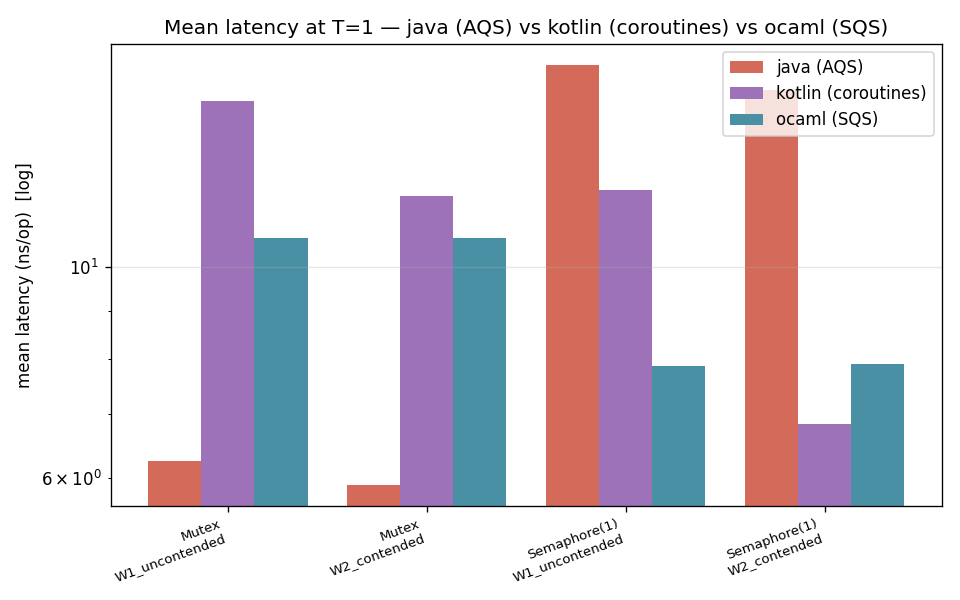
\includegraphics[width=0.49\linewidth]{mean_latency_T1.png}\hfill
  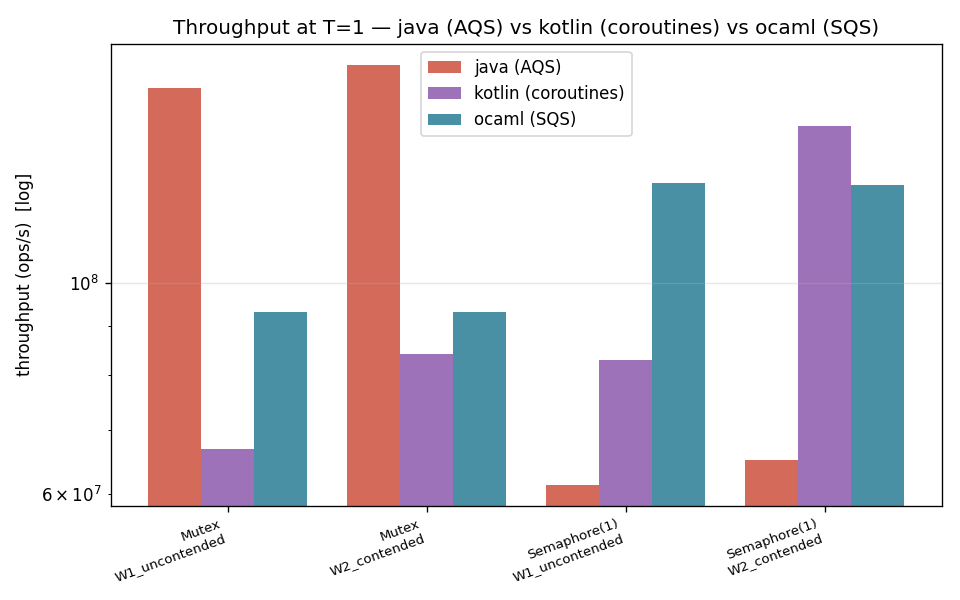
\includegraphics[width=0.49\linewidth]{throughput_T1.png}\\[0.6em]
  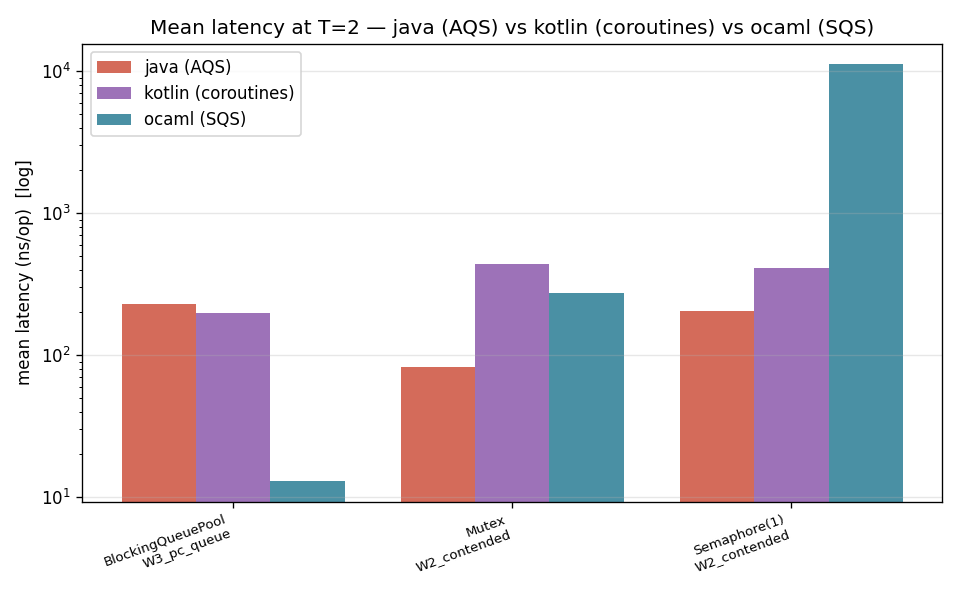
\includegraphics[width=0.49\linewidth]{mean_latency_T2.png}\hfill
  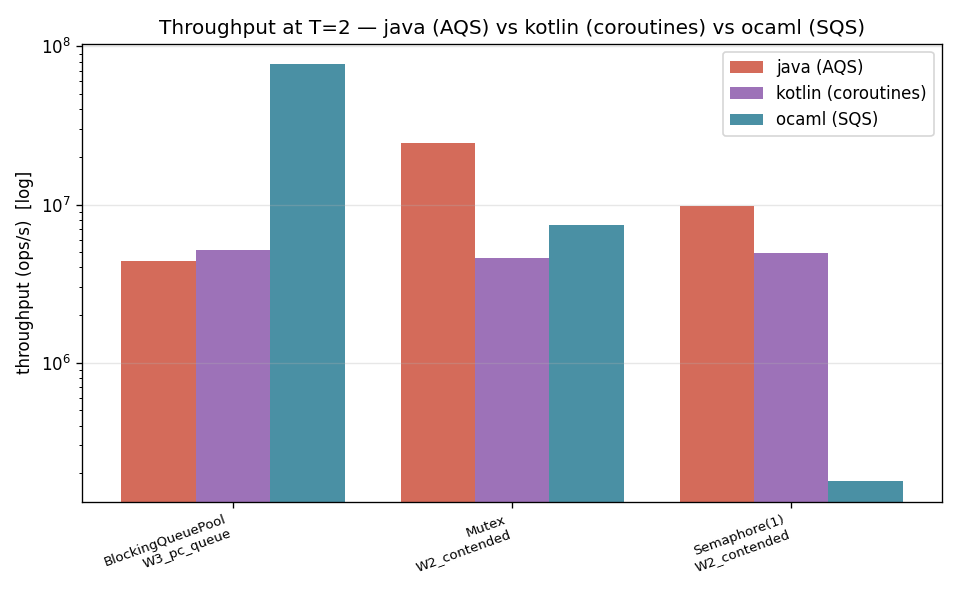
\includegraphics[width=0.49\linewidth]{throughput_T2.png}\\[0.6em]
  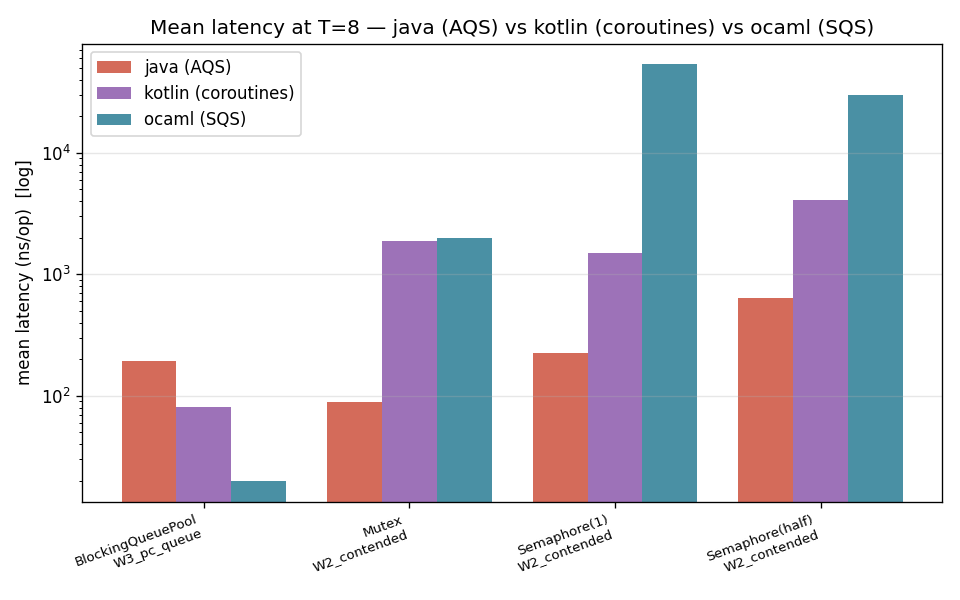
\includegraphics[width=0.49\linewidth]{mean_latency_T8.png}\hfill
  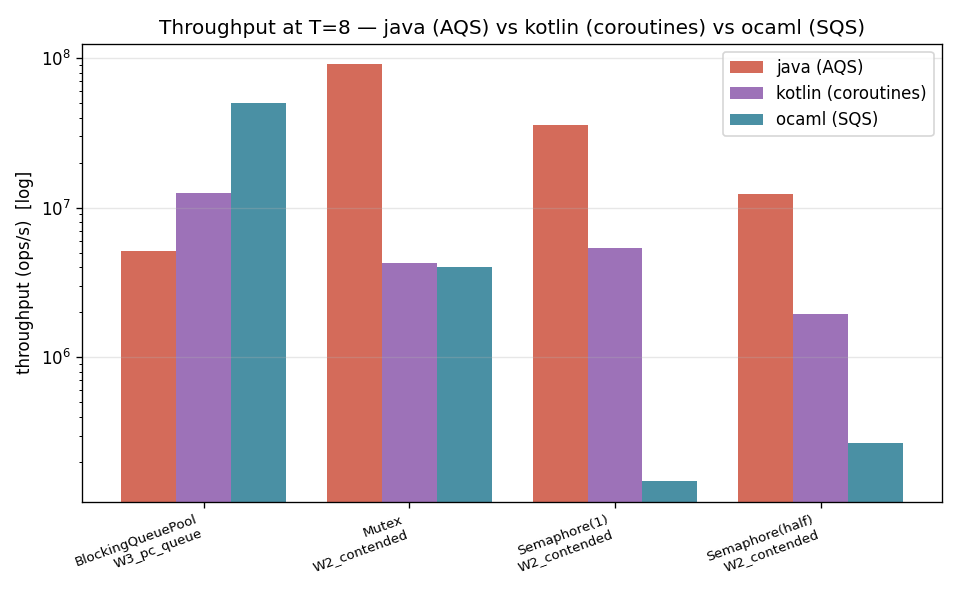
\includegraphics[width=0.49\linewidth]{throughput_T8.png}
  \caption{Mean per-op latency (ns, left column) and throughput
  (ops/s, right column) per primitive, with rows pinned to thread
  counts \texttt{T=1, 2, 8} (top to bottom). \texttt{T=1} is the
  uncontended fast path; \texttt{T=2}, \texttt{T=8} force
  cross-domain hand-off on the contended workloads.}
  \label{fig:lat-tput-grid}
\end{figure}


\subsubsection{What the numbers say}
\label{sec:eval-numbers}

Two patterns dominate. First, on the producer-consumer workloads
(\texttt{W3\_pc\_queue}, \texttt{W4\_pc\_stack}) and on the latch-fire
and barrier workloads (\texttt{W5\_latch\_fire}, \texttt{W6\_barrier}),
the OCaml SQS-backed primitives match or beat the Java
\texttt{java.util.concurrent} baseline: per-op latencies in the
$10\text{--}25\,\text{ns}$ band against $130\text{--}400\,\text{ns}$
for Java's \texttt{LinkedBlockingQueue}. Second, on contended
single-permit primitives (\texttt{Mutex} and \texttt{Semaphore(1)}
under \texttt{W2\_contended}), the picture inverts: OCaml is slower
than Java by $3\text{--}50\times$ depending on threads, with
\texttt{Semaphore(1)} \texttt{T=2} measuring $\approx 9.6\text{--}11.8\,\mu\text{s/op}$
on OCaml against $\approx 145\text{--}211\,\text{ns/op}$ on Java, per
\texttt{benchmark/results/summary.csv}.

\subsubsection{Why the numbers look this way}
\label{sec:eval-reasons}

The two patterns have a single underlying cause: where the cost lives.
We enumerate the contributing reasons explicitly.

\begin{enumerate}
\item \textbf{Eio per-domain event-loop wake-up vs.\ JVM
  \texttt{LockSupport.park}/\texttt{unpark}.} Each OCaml domain runs
  its own \texttt{Eio\_main.run} (\texttt{benchmark/ocaml/bench.ml:63,~93}).
  When \texttt{Semaphore.release} on domain $A$ must wake an
  \texttt{acquire} parked on domain $B$, the wake-up traverses Eio's
  domain-safe enqueue $\rightarrow$ target run-queue $\rightarrow$ next
  scheduler poll. The JVM directly unparks the OS thread via the
  kernel-level park primitive. This indirection is the dominant cost
  on contended single-permit primitives and explains the
  \texttt{Semaphore(1)} \texttt{T=2} 50$\times$ gap (Java
  $\approx 145\text{--}211\,\text{ns}$, OCaml
  $\approx 9\,600\text{--}11\,800\,\text{ns}$).

\item \textbf{\texttt{java.util.concurrent.locks.ReentrantLock} is
  reentrant and has a thread-local owner cache; our \texttt{Mutex}
  has neither.} The SQS \texttt{Mutex}
  (\texttt{implementations/mutex.ml}) was refactored in commit
  \commit{67d3eed} to introduce a TTAS fast path: uncontended
  \texttt{lock} is a single \texttt{CAS} on a \texttt{bool Atomic.t},
  and uncontended \texttt{unlock} writes \texttt{false} and reads a
  \texttt{waiters} counter-if zero, the SQS is not touched at
  all. The \texttt{T=1} mutex row ($\approx 10.7\,\text{ns/op}$ in
  \texttt{summary.csv}) is the cost of that fast path: one CAS, one
  store, one load. Java's \texttt{ReentrantLock} at \texttt{T=1}
  ($\approx 5.8\,\text{ns/op}$) still wins because its thread-local
  owner cache makes a re-acquire from the same thread cheaper than a
  CAS, and it supports reentrancy and adaptive spin-then-park under
  contention. Under contention the SQS \texttt{Mutex} slow path
  increments \texttt{waiters}, parks via \texttt{suspend}, and
  retries the CAS on wake-up (a barging-allowed loop, matching
  \texttt{ReentrantLock(false)}); the cross-domain handoff cost of
  reason~(1) dominates from \texttt{T=2} onward. The \texttt{Mutex
  W2} row therefore compares apples-to-oranges; we additionally show
  \texttt{Semaphore(1)} precisely because it is the closer
  like-for-like.

\item \textbf{Java's \texttt{LinkedBlockingQueue} acquires a
  \texttt{ReentrantLock} on every \texttt{put}/\texttt{take} regardless
  of queue state.} That is $\approx 130\text{--}400\,\text{ns}$ of
  lock acquire+release per op even on a hot queue. Our
  \texttt{Blocking\_queue\_pool.put}
  (\texttt{implementations/blocking\_queue\_pool.ml:58--66}) and
  \texttt{retrieve} (\texttt{:78--88}) are lock-free in the steady
  state: one \texttt{Atomic.fetch\_and\_add} plus one
  \texttt{Atomic.compare\_and\_set} or \texttt{Atomic.exchange} on a
  \texttt{slot\_count = 1024} atomic array. With a hot queue the SQS
  \texttt{suspend} path is never invoked, so the cost reduces to two
  atomics, $\approx 12\text{--}22\,\text{ns}$. This is the inversion
  visible in \cref{fig:lat-tput-grid}.

\item \textbf{Kotlin's \texttt{Channel<T>(UNLIMITED)} adds coroutine
  state-machine overhead per \texttt{send}/\texttt{receive.}} The
  single Kotlin row currently in \texttt{summary.csv}
  (\texttt{Semaphore(1) W2 T=1}, $\approx 6.8\,\text{ns}$) is
  uncontended. Under contention coroutine dispatch cost would
  compound on top of reason~(1): the suspending channel goes through
  the dispatcher thread pool to resume the receiver, with the same
  cross-OS-thread wake-up nature as Eio's cross-domain enqueue but
  with additional state-machine bookkeeping per resume.

\item \textbf{Single-permit serialisation in \texttt{W2\_contended}.}
  \texttt{Semaphore(1)} forces every operation through one cell of the
  SQS infinite array, so all contention in the test serialises. The
  added \texttt{Semaphore(half)} run (commit \commit{3165e99},
  \texttt{T=4} and \texttt{T=8}) lets $t/2$ acquirers proceed in
  parallel while the other $t/2$ park, spreading the wake-up cost
  across multiple cells. The smaller \texttt{Semaphore(half)} latency
  vs.\ \texttt{Semaphore(1)} at the same thread count confirms the
  bottleneck is the cross-domain handoff, not the cell-state machine
  itself.

\item \textbf{Domain creation and teardown cost is included in
  \texttt{W5\_latch\_fire} and \texttt{W6\_barrier.}} These workloads
  create a fresh \texttt{CountDownLatch} or \texttt{Barrier} per cycle
  (\texttt{benchmark/README.md}); the Java side mirrors the cycle
  shape so the comparison is fair, but absolute numbers in those rows
  reflect setup overhead and cannot be read as steady-state primitive
  cost.


\end{enumerate}

\subsection{Limitations of the evaluation}
\label{sec:eval-limitations}

The numbers above were gathered on one machine, under one kernel
scheduler, with mean-latency reporting only and no isolation between
Eio scheduler overhead and raw \texttt{Domain.spawn} overhead (we use
one domain per measured thread). Java's JIT may still be in tier-2
compilation early in our 1\,s warm-up window for the lower-thread
cells. Cross-machine variance, p99/p999 latency, and a separate
``no-Eio'' baseline (raw atomics + \texttt{Mutex.t} from
\texttt{Stdlib.Mutex}) are obvious next steps but were out of scope.

% =============================================================================
\section{Reflection on the Use of LLMs}
\label{sec:llm}
% =============================================================================

\paragraph{Tools.} We initially started our implementation using Claude Sonnet
which used simple closures. However, we then switched to using effect handlers
and continuations since we required cancellable API. With the help of Cluade
Opus, we were able to figure out that these continuations weren't thread safe
and from there Opus was able to suggest Eio.Fiber which provided
Eio.Fiber.Cancel, porting over our entire codebase to use OCaml/Eio. Opus,
running through Claude Code, also helped create a new test scaffolding, and
implemented the benchmark drivers from scratch looking at Kotlin codebase, after
we moved off Sonnet. In the midst, we also relied on ChatGPT Codex (GPT-5) for
extracting from the paper and explaining parts of it.

\paragraph{What worked.} The best results came when describing our tasks in
phased prompts, and using \emph{Plan} mode for larger tasks. Early smoke tests
and sanity checks helped ensure that we were going in the right direction. Using
the templates from assignments for qcheck-lin and qcheck-stm helped make sure
Claude Code doesn't go astray while trying to create a harness and improved the
output quality by keeping things simple and easy to parse. Human-in-the-loop
discussion and reading through the thinking logs were essential for selecting
optimisations and the Eio alternative.

\paragraph{What did not.} Claude Sonnet actually silently dropped the
\texttt{REFUSED} state from the \texttt{Cell} data structure when initially
porting from Kotlin, breaking correctness and forcing a repo-wide rewrite using
Opus. However, even Opus was not immune: a test started failing because the
configured \texttt{Semaphore(1)} whereas the test required
\texttt{Semaphore(2)}, producing a deadlock that had to be diagnosed by hand. In
addition, supplying PDF inputs inflated token use without commensurate gain.

\paragraph{What surprised us.} The agents recovered well when reframed. Thinking
logs of CLAUDE helped show that the early effect-handler design for light
threads was unsafe across domains (continuations are domain-local, especially
under cancellation); once the problem was posed precisely, Opus pivoted to the
Eio domain-safe enqueue design that the final implementation now uses.

\paragraph{What was hard.} Communication with Opus, and choosing the correct
amount of verbosity in prompts, were both challenging. Explaining benchmark
results was the hardest part.We had to tell the agent that Java's
\emph{ReentrantLock} is reentrant (so the contended-mutex numbers were not an
apples-to-apples comparison with our non-reentrant SQS mutex), and that the
producer-consumer pool numbers looked too good because the OCaml run was hitting
the fast path. The agent will not notice these things unless you point them out.

\paragraph{Assessment.}
Agentic LLMs accelerated the port substantially but stayed highly
sensitive to prompt quality and weak at preserving subtle correctness
invariants; rigorous human review remained necessary.

% =============================================================================
\section{Conclusions}
\label{sec:conclusions}
% =============================================================================

CQS framework translates cleanly to OCaml~5 + Eio, but the results are mixed.

The lock-free fast path that buys us time on producer-consumer queues, latch-fire, and barriers but costs us  on \texttt{Mutex} and \texttt{Semaphore(1)} under contention. Our multi-layer testing strategy (lin harness, \texttt{qcheck-lin}, \texttt{qcheck-stm}, manual scenarios, TSAN) caught a distinct class of bug at each layer (\cref{sec:tasks-bugs}), however (\cref{sec:tasks-test-gaps}) -  the nine-state cell machine is not asserted directly, \texttt{Sync} mode and \texttt{Broken} are unreachable from production primitives, cancellation paths are exercised only indirectly and benchmarks are only single machines.

Given more time we would expose an internal cell accessor so \texttt{qcheck-stm} can model the cell machine directly, attack the cross-domain wake-up cost (Eio-side same-domain bypass or primitive-level adaptive spin), broaden the benchmarks (p99/p999, raw \texttt{Stdlib.Mutex} baselines, x86).





% =============================================================================
\section*{Contributions}
\label{sec:contributions}
% =============================================================================

% Required. Percentages must sum to 100. Every member should contribute.

\begin{center}
\begin{tabular}{@{}lc>{\raggedright\arraybackslash}p{0.45\linewidth}@{}}
\toprule
\textbf{Member} & \textbf{Contribution (\%)} & \textbf{Main responsibilities} \\
\midrule
Mitesh Sharma         & 40\% &  CQS Core implementations, Revisions with Effect Handlers, Eio.Fiber integration, Async Primitive implementations\\
Navaneeth M Nambiar & 30\% &  Developing QCheck-Lin tests and STM for implementations, Project Refactoring while keeping the regressions minimal\\
Durwasa Chakraborty   & 30\% & Benchmarking suite with Java and Kotlin, Graph generation, Report compilation \\
\midrule
\textbf{Total}        & \textbf{100\%} & \\
\bottomrule
\end{tabular}
\end{center}

% =============================================================================
\bibliographystyle{plainurl}
\bibliography{references}
% =============================================================================

\end{document}
